% !TEX root = dta.tex
\lipsum[3]

\section{Latar Belakang}
\lipsum[10-11]
\begin{equation}
  \int^b_a (f(x)+g(x)) \, dx = \int^b_a f(x)\, dx + \int^b_a g(x) \, dx
\end{equation}
\lipsum[90]


\begin{figure}[H]
  \centering
  \label{fig:skema}
  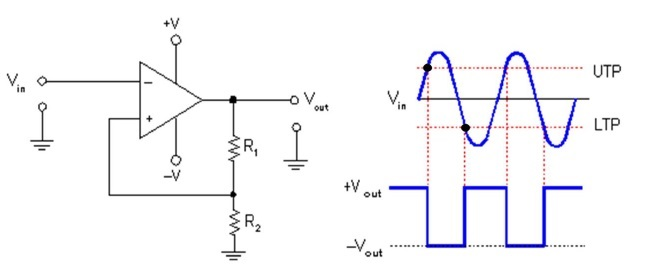
\includegraphics[width=.8\textwidth]{img/skema.jpg}
  \caption{Contoh Input Gambar}
\end{figure}

\section{Rumusan Masalah}
\lipsum[88]\cite{book1,book2}
